\chapter{GrShell Language}
\label{chapgrshell}

The \GrShell\ is a shell application of the \LibGr. It belongs to \GrG's standard equipment. \GrShell\ is capable of creating, manipulating and dumping graphs as well as performing graph rewriting and debugging graph rewriting.

The \GrShell\ language is a line oriented scripting language. It is structured by simple statements separated by line breaks.

\section{Building Blocks}

The \GrShell\ is case sensitive. A comment starts with a \emph{\#} and is terminated by end-of-line or end-of-file. Any text left of the \emph{\#} will be treated as a statement.

\begin{rail} 
 Text : '<DoubleQuotedText>' | '<SingleQuotedText>' | '<Word>' ;
 Number : '<Number>' ;
 TextOrNumber : Text | Number ;
 Parameters : Text + ',' ;
 SpacedParameters: Text + ; 
\end{rail}

Those items are required for representing text, numbers and parameters within rules. The tokens \verb+<...>+ are defined as follows:\\

\begin{tabularx}{\linewidth}{lX}
\verb+<$Word$>+:            & A character sequence consisting of letters, digits and underscores. The first character must not be a digit.\\
\verb+<DoubleQuotedText>+:  & Arbitrary text enclosed by double quotes (`` '').\\
\verb+<SingleQuotedText>+:  & Arbitrary text enclosed by single quotes (` ').\\
\verb+<Number>+:            & A sequence of digits.
\end{tabularx}\\

In order to describe the possible input to some of the commands more precisely, the following (semantic) specializations of \emph{Text} are defined:\\

\begin{tabularx}{\linewidth}{lX}
Filename: & A file path without spaces (e.g.\ /Users/Bob/amazing\textunderscore file.txt) or a single quoted or double quoted file path that may contain spaces (``/Users/Bob/amazing\textunderscore file.txt'').\\
Variable: & Identifier of a variable that contains a graph element.\\
NodeType: & Identifier of a node type within the model of the current graph.\\
AttributeName: & Identifier of an attribute.\\
Graph: & Identifies a graph by its name. \\
Action: & Identifies a rule by its name.\\
Color: & One of the following color identifiers: Black, Blue, Green, Cyan, Red, Purple, Brown, Grey, LightGrey, LightBlue, LightGreen, LightCyan, LightRed, LightPurple, Yellow, White, DarkBlue, DarkRed, DarkGreen, DarkYellow, DarkMagenta, DarkCyan, Gold, Lilac, Turquoise, Aquamarine, Khaki, Pink, Orange, Orchid. These are the same color identifiers as in VCG/\yComp\ files.
\end{tabularx}\\

The elements of a graph (nodes and edges) can be accessed both by their variable identifier and by their persistent name specified through a constructor (see \ref{mani}):
\makeatletter
\begin{rail}
  GraphElement: Text | ('@' '(' Text ')')
\end{rail}
\makeatother
The specializations \emph{Node} and \emph{Edge} of \emph{GraphElement} requires the corresponding graph element to be a node or an edge respectively.
\begin{example}
\label{persistentex} 
We insert a node, anonymously and with a constructor:
\begin{grshell}
> select backend lgspBackend.dll
Backend selected successfully.
> new graph "../lib/lgsp-TuringModel.dll" G
New graph "G" of model "Turing" created.
  
# insert an anonymous node... 
# it will get a persistent pseudo name
> new :State  
New node "$0" of type "State" has been created.
> delete node @("$0")
  
# and now with constructor
> new v:State($=start) 
new node "start" of type "State" has been created.
# Variable v is now assigned to start
> new :State($=end)
new node "end" of type "State" has been created.
  
# actually we want v to be "end": 
>  v = @(end)
>
\end{grshell}
\end{example}
\begin{note}
Persistent names belong to a specific graph, whereas variables belong to the current \GrShell\ environment. Persistent names will be saved (\texttt{save graph\dots}, see \ref{outputcmds}) and, if you visualize a graph (\texttt{dump graph\dots}, see \ref{outputcmds}), graph elements will be labeled with their persistent names. Persistent names have to be unique for a graph.
\end{note}

\begin{rail}
  Variable '=' GraphElement   
\end{rail}
Assigns the variable or persistent name \emph{GraphElement} to \emph{Variable}. If \emph{Variable} has not been defined yet, it will be defined implicitly. As usual for scripting languages, variables have neither types nor declarations.

\section{\GrShell\ Commands}
This section describes the \GrShell\ commands. Commands are assembled from basic elements. As stated before commands are terminated by a line breaks. Alternatively commands can be terminated by the \texttt{;;} symbol.
\begin{rail}
  Script: ((Command ('<line break>' | ';;'))+) '<end of file>' ;
\end{rail}

\subsection{Common Commands}
\label{commcommands}
\begin{rail}
  'help'
\end{rail}
Displays an information message describing supported commands. 

\begin{rail}
  'quit' | 'exit'
\end{rail}
Quits \GrShell. If \GrShell\ is opened in debug mode, currently active graph displayers (such as \yComp) will be closed as well.

\begin{rail}
  'select' 'backend' Filename ( ( ) | ':' Parameters )
\end{rail}
Selects a backend that handles graph and rules representation. \emph{Filename} has to be a .NET assembly (e.g.\ ``lgspBackend.dll'').  Comma-separated parameters can be supplied optionally. If so, the backend must support these parameters.

\begin{rail}
  'show' 'backend' Filename
\end{rail}
List all the parameters supported by the backend \emph{Filename}, that can be provided to the \texttt{select backend} command.

\begin{rail}
  'include' Filename
\end{rail}
Executes the \GrShell\ script \emph{Filename}. A \GrShell\ script is just a plain text file containing \GrShell\ commands. They are treated as they would be entered interactively, except for parser errors. If an parser error occurs, execution of the script will stop immediately.

\begin{rail}
  'debug' ( 'enable' | 'disable' )
\end{rail} 
Enables and disables the debug mode. The debug mode shows the current working graph in a \yComp\ window. All changes to the working graph are tracked by \yComp\ immediately.  

\begin{rail}
  'echo' Text
\end{rail}
Prints \emph{Text} onto the \GrShell\ command prompt.

\subsection{Graph Commands}
\label{graphcommands}

\begin{rail}
  'new' 'graph' Filename Text 
\end{rail}
Creates a new graph with the model specified in \emph{Filename}. Its name is set to \emph{Text}. The model file can be either source code (e.g.\ ``turing\textunderscore machine.cs'') or a .NET assembly (e.g.\ ``turing\textunderscore machine.dll'').

\begin{rail}
  'open' 'graph' Filename Text
\end{rail}
Opens the graph \emph{Text} stored in the backend. Its model is specified in \emph{File\-name}. However, the \emph{LGSPBackend} doesn't support persistent graphs. \emph{LGSPBackend} is the only backend so far. Therefore this command is useless at the moment.

\begin{rail}
  'show' 'graphs'
\end{rail}
Displays a list of currently available graphs.

\begin{rail}
  'select' 'graph' Graph
\end{rail}
Selects the current working graph.

\begin{rail}
  'delete' 'graph' Graph
\end{rail}
Deletes the graph \emph{Graph} from the backend storage.

\begin{rail}
  'validate' ( ( ) | 'strict' )
\end{rail}
Validates if the current working graph fulfills the edge constraints specified in the corresponding graph model. The \emph{strict} mode additionally requires all the edges of the working graph to be specified in order to get a ``valid''. Otherwise edges between nodes without specified constraints are ignored.\\
\begin{example}
We reuse a simplified version of the street map model from chapter \ref{chapmodellang}:
\begin{grgen} 
model Map;

node class city;
node class metropolis;

edge class street;
edge class highway
      connect metropolis [+] -> metropolis [+];
\end{grgen}
The node constraint on \emph{highway} requires all the metropolises to be connected by highways. Now have a look at the following graph:
\begin{center}
  \fbox{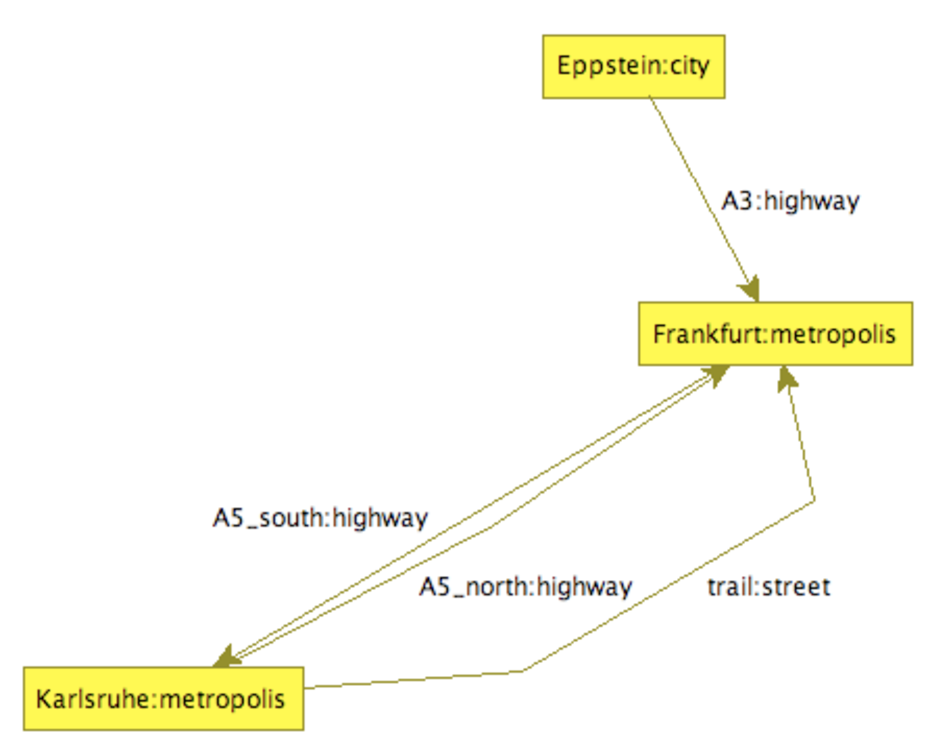
\includegraphics[width=8.5cm]{fig/map}}
\end{center}

This graph is valid, but not strict valid.
\begin{grshell} 
> validate
The graph is valid.
> validate strict
The graph is NOT valid:
  CAE: city "Eppstein" -- highway "A3" --> metropolis "Frankfurt" not specified
  CAE: metropolis "Karlsruhe" -- street "trail" --> metropolis "Frankfurt" not specified
>
\end{grshell}
\end{example}

\begin{rail}
  'custom' 'graph' ( ( ) | SpacedParameters )
\end{rail}
Executes a command specific to the current backend. If \emph{SpacedParameters} is omitted, a list of available commands will be displayed (for the LGSP backend see \ref{custom}).

\subsection{Graph Manipulation Commands}
\label{mani}
In order to create graph elements an optional constructor can be used. 
\begin{rail}
  Constructor : '(' (() | (dollar '=' Text (() | ',' Attributes) | Attributes)) ')';
  Attributes : SingleAttribute + ',' ;
  SingleAttribute : AttributeName '=' TextOrNumber ; 
\end{rail}
A comma separated list of attribute declarations is supplied to the constructor. Available attribute names are specified by the graph model of the current working graph. All the undeclared attributes will be initialized with default values, depending on their type (int, enum $\leftarrow$ 0; boolean $\leftarrow$ false; float, double 0.0; string $\leftarrow$ ``'').\\
The \texttt{\$} marks a special attribute: an unique identifier of the new graph element. This identifier also is denoted as \emph{persistent name} (see \ref{persistentex}, \emph{GraphElement}). This name can be specified by a constructor only.

\begin{rail}
  'new' (() | Text) (() | ':' NodeType (() | Constructor))
\end{rail}
Creates a new node within the current graph. Optionally a variable \emph{Text} is assigned to the new node. If \emph{NodeType} is supplied, the new node will be of type \emph{NodeType} and attributes can be initialized by a constructor. Otherwise the node will be of the base node class type \emph{Node}.

\begin{rail}
  'new' Node '-' (()|Text) \\ (() | ':' EdgeType (() | Constructor)) '->' Node
\end{rail}
Creates a new edge within the current graph between the specified nodes, directed towards the second \emph{Node}. Optionally a variable \emph{Text} is assigned to the new edge. If \emph{EdgeType} is supplied, the new edge will be of type \emph{EdgeType} and attributes can be initialized by a constructor. Otherwise the edge will be of the base edge class type \emph{Edge}.

\begin{rail}
  GraphElement '.' AttributeName '=' TextOrNumber
\end{rail}
Set the attribute \emph{AttributeName} of the graph element \emph{GraphElement} to the value of \emph{TextOrNumber}.

\begin{rail}
  'delete' 'node' Node
\end{rail}
Deletes the node \emph{Node} from the current graph. Incident edges will be deleted as well.

\begin{rail}
  'delete' 'edge' Edge
\end{rail}
Deletes the edge \emph{Edge} from the current graph.  
  
\subsection{Graph Query Commands}

\begin{rail}
  'show' (() | 'num') ('nodes' (() | NodeType) | 'edges' (() | EdgeType))
\end{rail}
Gets the persistent names and the types of all the nodes / edges of the current graph. If a node type or edge type is supplied, only elements compatible to this type are considered. Nodes / edges without persistent names are shown with a pseudo-name.\\
If the command is specified with \texttt{num}, only the number of nodes/edges will be displayed.

\begin{rail}
  'show' ('node' | 'edge') 'types'
\end{rail}
Gets the node / edge types of the current graph model.

\begin{rail}
'show' ('node' ('super' | 'sub') 'types' NodeType | 'edge' ('super' | 'sub') 'types' EdgeType)
\end{rail}
Gets the inherited / descended types of \emph{NodeType} / \emph{EdgeType}.

\begin{rail}
  'show' ('node' 'attributes' (() | (() | 'only') NodeType) | 'edge' 'attributes' (() | (() | 'only') EdgeType))
\end{rail}
Gets the available node / edge attribute types. If \emph{NodeType} / \emph{EdgeType} is supplied, only attributes defined in \emph{NodeType} / \emph{EdgeType}. The \texttt{only} keyword excludes inherited attributes.\\
\begin{note}
This is in contrast to the \texttt{show num\dots}, \texttt{show nodes\dots} and \texttt{show edges\dots} commands where types and \emph{sub}types are specified.
\end{note}

\begin{rail}
 'show' ('node' Node | 'edge' Edge)
\end{rail}
Gets the attribute types and values of a specific graph element.

\begin{rail}
  'show' GraphElement '.' AttributeName
\end{rail}
Gets the value of a specific attribute.

\begin{rail}
  'node' 'type' Node 'is' Node | 'edge' 'type' Edge 'is' Edge
\end{rail}
Gets the information, whether the first element is type-compatible to the second element.

\subsection{Graph Output Commands}
\label{outputcmds}

\begin{rail}
  'save' 'graph' Filename
\end{rail}
Dumps the current graph as \GrShell\ script into \emph{Filename}. The created script includes
\begin{itemize}
  \item selecting the backend
  \item creating all nodes and edges
  \item restoring the persistent names (see \ref{mani}),
\end{itemize}
but not necessarily using the same commands you typed in during construction.

\begin{rail}
  'show' 'graph' Filename (() | Text)
\end{rail}
Dumps the current graph as VCG formatted file into a temporary file. \emph{Filename} specifies an executable. The temporary VCG file will be passed to \emph{Filename} as last parameter. Additional parameters, such as program options, can be specified by \emph{Text}. If you use \yComp\ as executable, this may look like
\begin{center}
  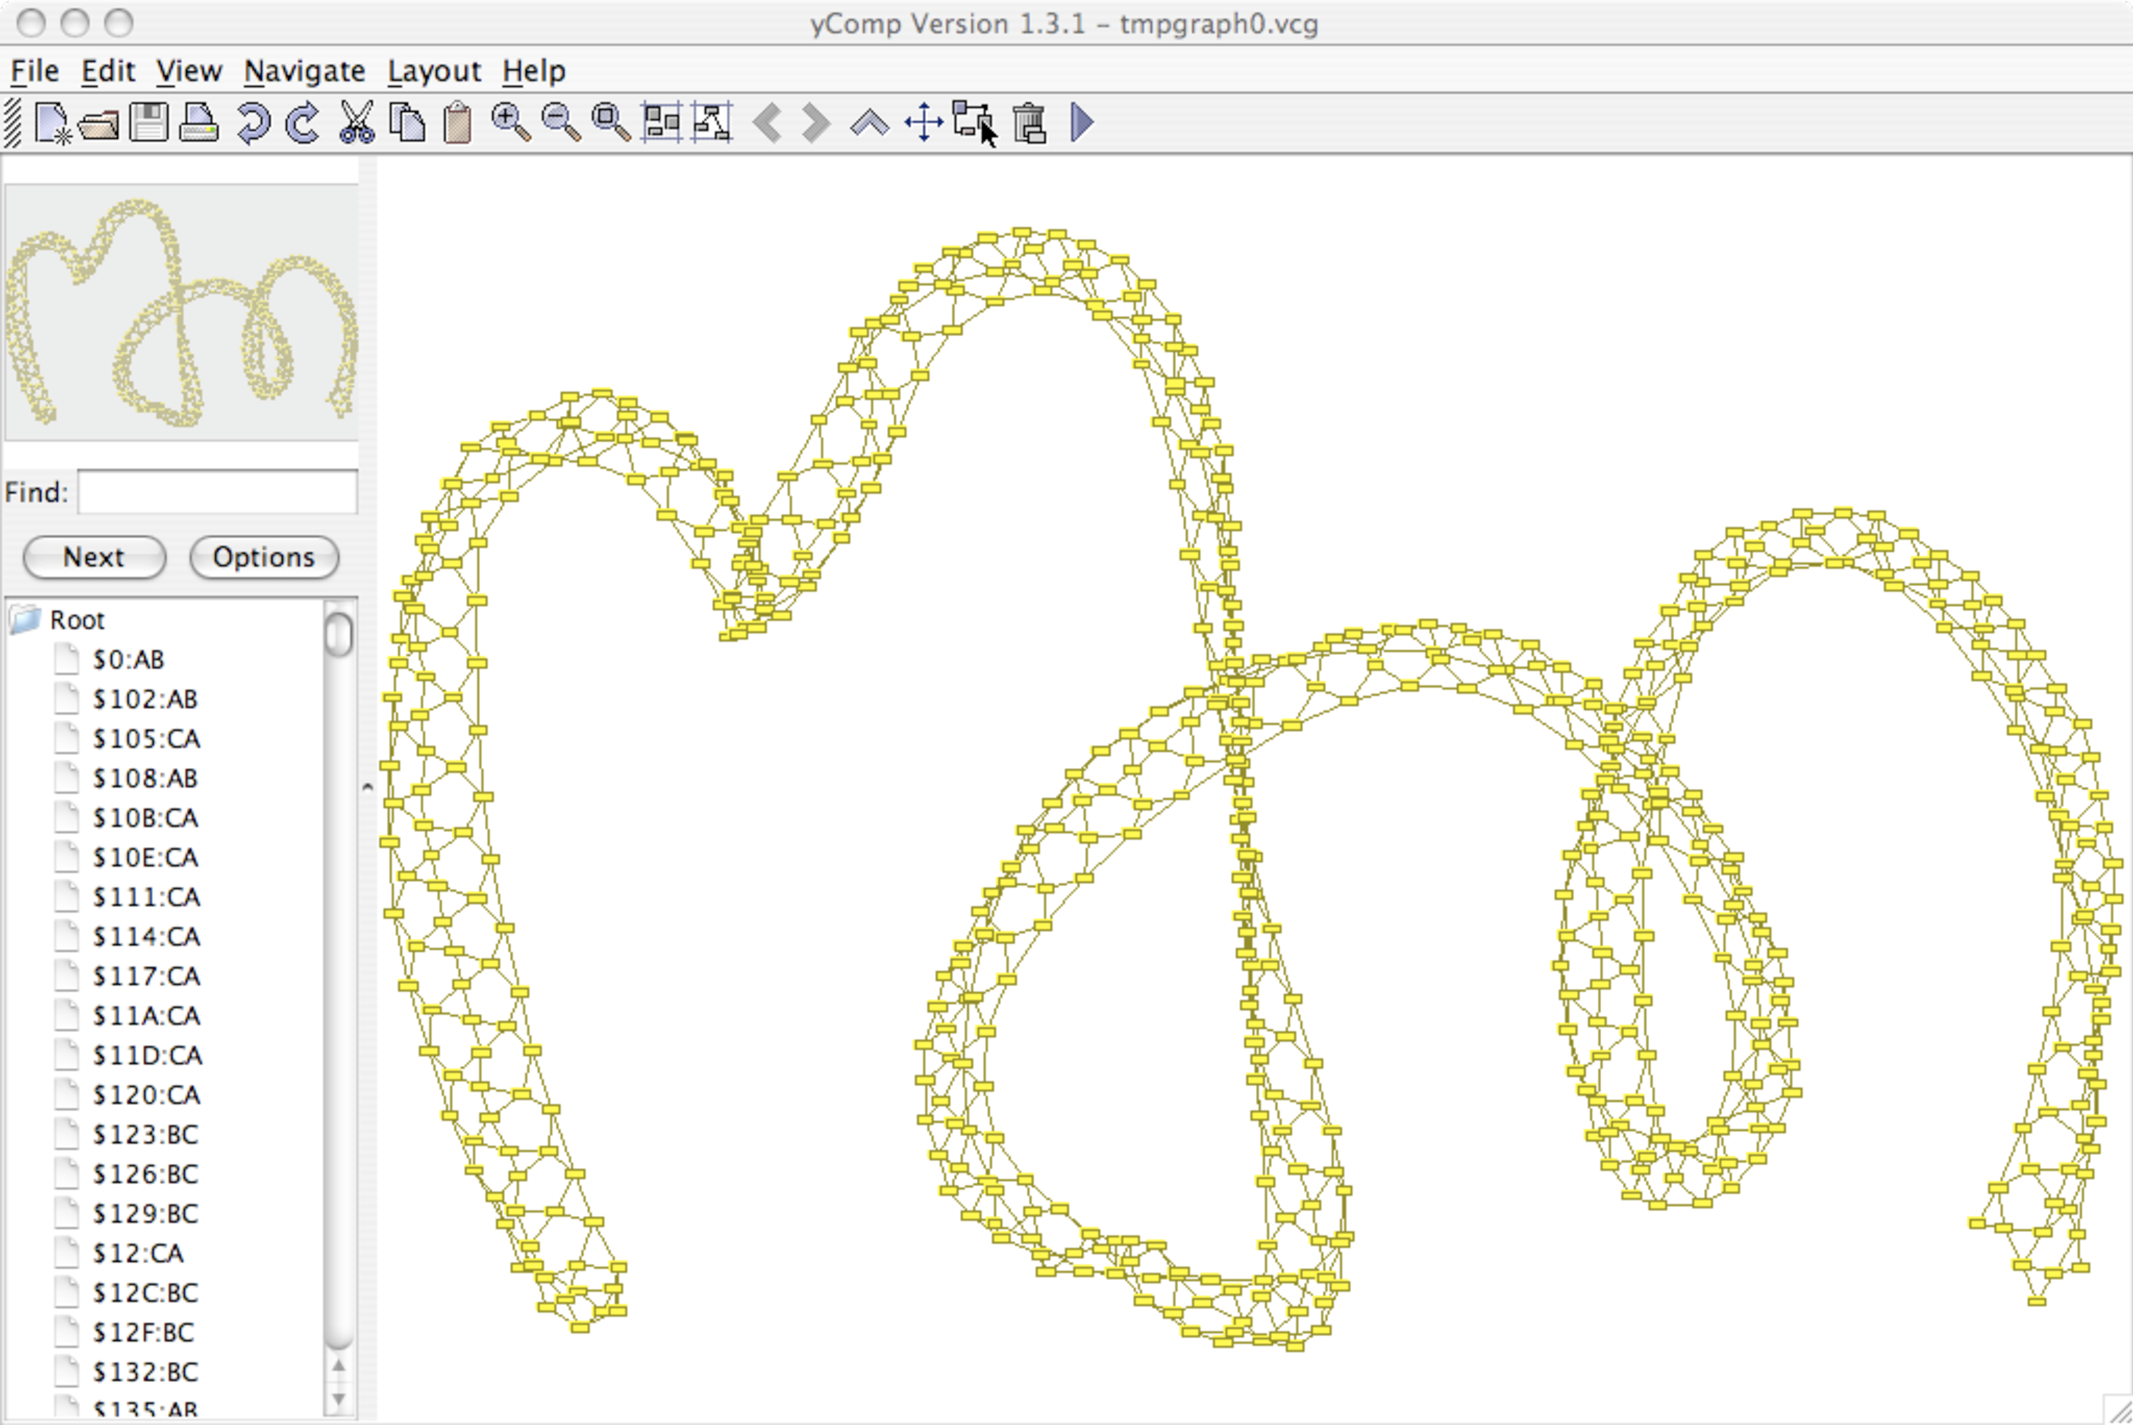
\includegraphics[width=0.75\linewidth]{fig/showgraph}
\end{center}  
The temporary file will be deleted, when \emph{Filename} is terminated, if \GrShell\ is still running at this time.

\begin{rail}
  'dump' 'graph' Filename
\end{rail}
Dumps the current graph as VCG formatted file into \emph{Filename}.\\
\\
The following commands control the style of the VCG output. This affects \texttt{dump graph}, \texttt{show graph} and \texttt{enable debug}. 
\begin{rail}
  'dump' 'set' ('color' | 'textcolor' | 'bordercolor') 'node' NodeType '=' Color
\end{rail}
Sets the color / text color / border color of the nodes of type \emph{NodeType}. This doesn't include sub types of \emph{NodeType}.

\begin{rail}
  'dump' 'set' ('color' | 'textcolor') 'edge' EdgeType '=' Color
\end{rail}
Sets the color / text color of the edges of type \emph{EdgeType}. This doesn't include sub types of \emph{NodeType}.

\begin{rail}
  'dump' 'add' 'exclude' 'node' NodeType
\end{rail}
Excludes nodes of type \emph{NodeType} (or sub type of \emph{NodeType}) as well as their incident edges from output.

\begin{rail}
  'dump' 'add' 'group' 'node' NodeType
\end{rail}
Declares \emph{NodeType} (or sub type of \emph{NodeType}) as group node type. All the different typed nodes that points to a node of type \emph{NodeType} (i.e.\ there is a directed edge between such nodes) will be grouped and visibly enclosed by the \emph{NodeType}-node.
The following example shows \emph{metropolis} ungrouped and grouped:
\begin{center}
  \fbox{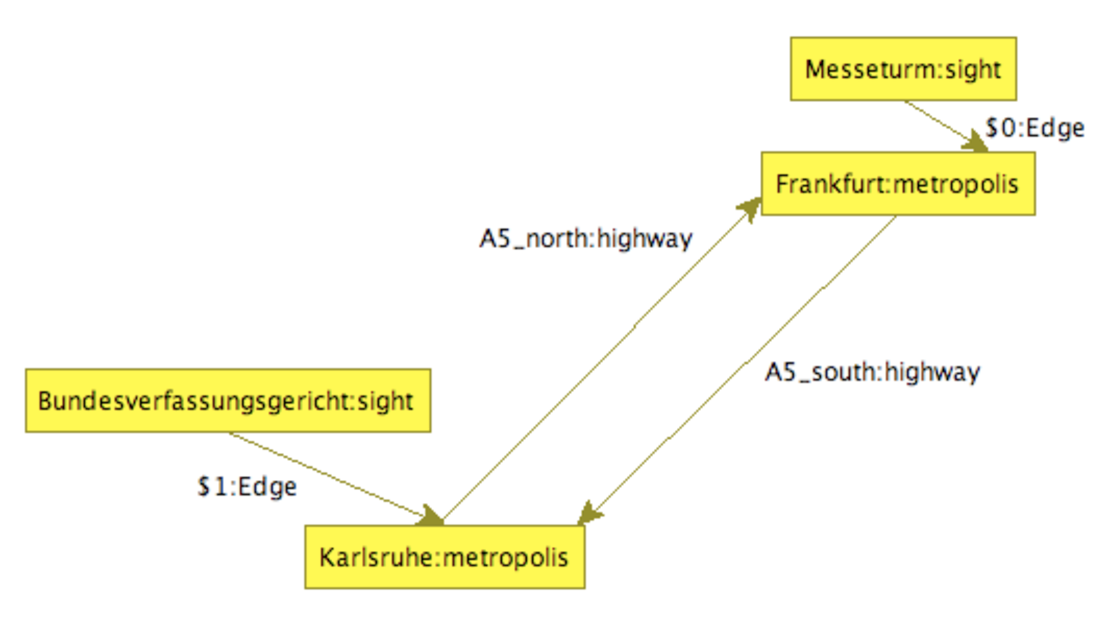
\includegraphics[width=0.45\linewidth]{fig/group1}}  \hfill \fbox{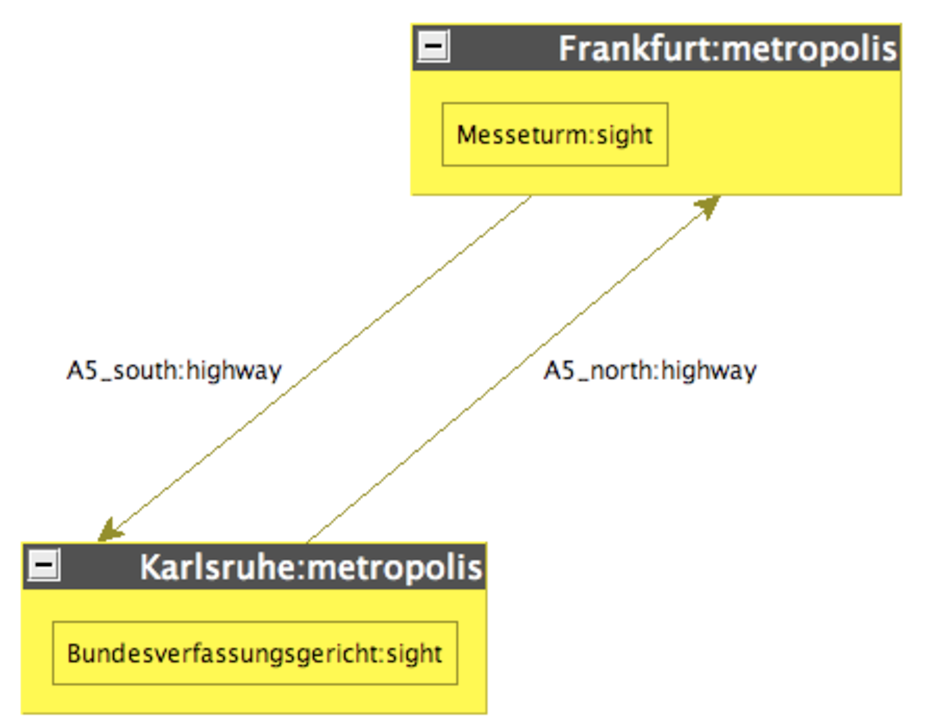
\includegraphics[width=0.45\linewidth]{fig/group2}}\\
  {\small right side: dumped with \texttt{dump add group node metropolis}}
\end{center}

\begin{rail}
  'dump' 'add' 'infotag' ('node' NodeType | 'edge' EdgeType) AttributeName
\end{rail}
Declares the attribute \emph{AttributeName} to be an ``info tag''. Info tags are displayed like additional node / edge labels. In the following example \emph{river} and \emph{jam} are info tags:
\begin{center}
  \fbox{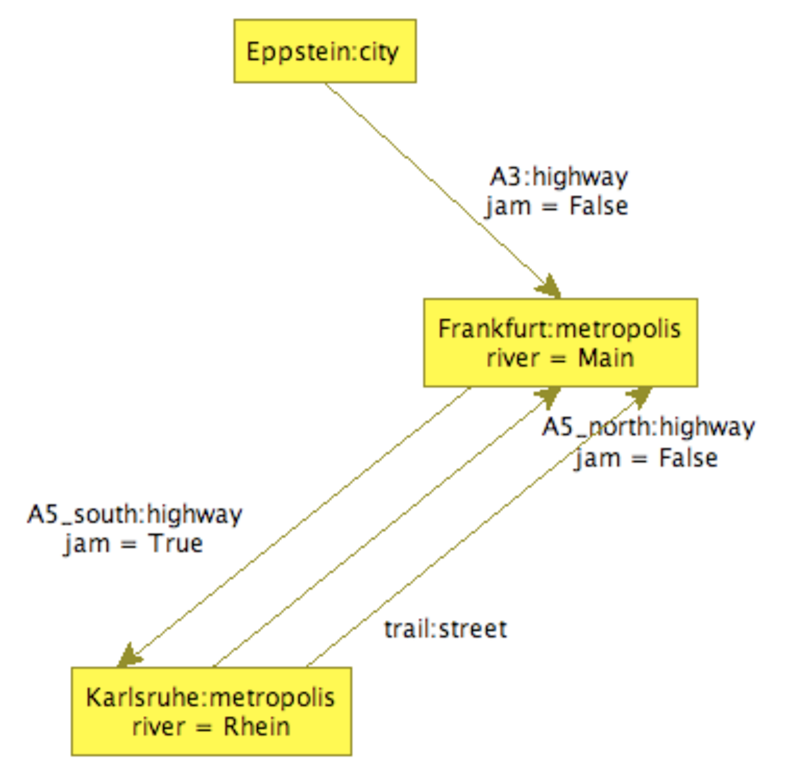
\includegraphics[width=0.5\linewidth]{fig/infotag}}
\end{center}


\begin{rail}
  'dump' 'set' 'edge' 'labels' ('on' | 'off')
\end{rail}
Specifies, whether edge labels will be displayed or not (default to ``on'').

\begin{rail}
  'dump' 'reset'
\end{rail}
Reset all style options (\texttt{dump set}\dots) to their default values.

\subsection{Action Commands (GRS)}
\label{grsthings}
An \emph{action} denotes a graph rewriting rule.

\begin{rail}
  'select' 'actions' Filename
\end{rail}
Selects a rule set. \emph{Filename} can be either a .NET assembly (e.g.\ ``rules.dll'') or a source file (``rules.cs''). Only one rule set can be loaded at once.

\begin{rail}
  'show' 'actions'
\end{rail}
Lists all the rules of the loaded rule set, their parameters and their return values. Rules can return a set of graph elements.

\begin{rail}
  'custom' 'actions' (() | SpacedParameters)
\end{rail}
Executes an action specific to the current backend. If \emph{SpacedParameters} is omitted, a list of available commands will be displayed (for the LGSPBackend see section \ref{custom}).

\subsubsection*{Regular Graph Rewrite Sequences}
Basically a graph rewriting command looks like this:
\makeatletter
\begin{rail}
  (() | 'debug') 'grs' SimpleRewriteSequence ;
  SimpleRewriteSequence: (SimpleTerm (() | ('*' | lbrace Number rbrace))) + ((() | dollar) (';' | '|' | ampersand));
  SimpleTerm: (() | '!') ('[' Rule ']' | Rule) |
    Text '=' (Text | '@' '(' Text ')') |
    'def' '(' Parameters ')' |
    'true' |
    'false' |
    '(' SimpleRewriteSequence ')' ;
  Rule: (() | '(' Parameters ')' '=') Action (() | '(' Parameters ')') ;
\end{rail}
\makeatother
\mbox{\quad}\\
Table \ref{ruletab} lists graph rewriting expressions at a glance. The operators hold the following order of precedence, starting with the lowest precedence: 
\[ \text{\texttt{;}} \;\;\;\;\;\;\; \text{\texttt{|}} \;\;\;\;\;\;\;  \text{\texttt{\&}}\] 
\makeatletter
\begin{table}[htbp]
\begin{minipage}{\linewidth} \renewcommand{\footnoterule}{} 
\begin{tabularx}{\linewidth}{|lX|}
\hline
\texttt{s ; t}		& \textbf{Concatenation.} First, \texttt{s} is executed, afterwards \texttt{t} is executed. The sequence \texttt{s ; t} is \emph{successfully} executed iff \texttt{s} or \texttt{t} is successfully executed.\\
\texttt{s | t}		& \textbf{XOR.} First, \texttt{s} is executed. Only if \texttt{s} fails, \texttt{t} is executed. The sequence \texttt{s | t} is successfully executed iff \texttt{s} or \texttt{t} is successfully executed.\\
\texttt{s \& t}	& \textbf{Transactional AND.} First, \texttt{s} is executed, afterwards \texttt{t} is executed. If \texttt{s} or \texttt{t} fails, the action will be terminated and a rollback to the state before \texttt{s \& t} is performed.\\
\texttt{\$<op>}	& Flags the operator \texttt{<op>} as commutative. Usually operands are executed / evaluated from left to right with respect to bracketing (left-associative). But the sequences \texttt{s}, \texttt{t}, \texttt{u} in \texttt{s \$<op> t \$<op> u} are executed / evaluated in arbitrary order. \\
\texttt{s *}		& Executes \texttt{s} repeatedly as long as its execution does not fail.\\
\texttt{s \{n\}}	& Executes \texttt{s} repeatedly as long as its execution does not fail, but anyway \texttt{n} times at most.\\
\texttt{!}		& Found matches are dumped into VCG formatted files. Every match produces three files within the current directoy\footnote{Make sure, that the path to your \texttt{yComp.jar} package is set correctly in the \texttt{ycomp} shell script within \GrG's \texttt{/bin} directory.}:
\begin{enumerate}
  \item The complete graph that has the matched graph elements marked
  \item The complete graph with additional information about matching details
  \item A subgraph containing only the matched graph elements
\end{enumerate}\\
\texttt{\emph{Rule}} & Only the first pattern match produced by the action \emph{Rule} will be rewritten.\\
\texttt{[\emph{Rule}]} & Every pattern match produced by the action \emph{Rule} will be rewritten. \textbf{Note:} This operator is mainly added for benchmark purposes. Its semantic is not equal to \texttt{Rule*}. Instead this operator collects all the matches first before starting rewritings. In particular one needs to avoid deleting a graph element that is bound by another match. \\
\texttt{v = w}	& The variable \texttt{v} is assigned to \texttt{w}. If \texttt{w} is undefined, \texttt{v} will be undefined, too.\\
\texttt{v = @(x)}	& The variable \texttt{v} is assigned to the graph element identified by \texttt{x}. If \texttt{x} is not defined any more, \texttt{v} will be undefined, too.\\
\texttt{def(\emph{Parameters})} & Gets \emph{successful} if all the graph elements in \emph{Parameters} exist, i.e.\ if all the variables are defined.\\
\texttt{true}	& A constant acting as a successful match.\\
\texttt{false}	& A constant acting as a failed match.\\ \hline
\end{tabularx}
\end{minipage}\\
\\ \centering
{\small Let \texttt{s}, \texttt{t}, \texttt{u} be graph rewriting sequences, \texttt{v}, \texttt{w} variable identifiers, \texttt{x} an identifier of a graph element, \texttt{<op>} $\in \{\texttt{;}, \texttt{|}, \texttt{\&}\}$ and \texttt{n} $\in \N_0$.}
\caption{Graph rewriting expressions}
\label{ruletab}
\end{table}
\makeatother

Variables can be assigned to graph elements returned by rules using \texttt{(\emph{Para\-meters}) = \emph{Action}}. The desired variable identifiers have to be listed in \emph{Parameters}. Graph elements required by rules must be provided using \texttt{\emph{Action} (\emph{Para\-meters})}, where \emph{Parameters} is a list of variable identifiers. For undefined variables the specific element constraint of \emph{Action} will be ignored (every element matches).\\

Use the \texttt{debug} option to trace the rewriting process step-by-step. During execution \yComp\ will display every single step\footnote{Make sure, that the path to your \texttt{yComp.jar} package is set correctly in the \texttt{ycomp} shell script within \GrG's \texttt{/bin} directory.}. The debugger can be controlled by \GrShell. The debug commands are shown in table \ref{tabdebug}.\\
\begin{table}[htbp]
  \begin{tabularx}{\linewidth}{|lX|} \hline
  \texttt{s}(tep) & Executes the next rewriting rule (match and rewrite)\\
  \texttt{d}(elaied step) & Executes a rewriting rule in a three-step procedure: matching, highlighting elements to be changed, doing rewriting \\
  \texttt{n}(ext) & Ascends one level up within the Kantorowitsch tree of the current rewrite sequence\\
  (step) \texttt{o}(ut) & Continues a rewriting sequence until the end of the current loop. If the execution is not in a loop at this moment, the complete sequence will be executed\\
  \texttt{r}(un) &  Continues execution without further stops\\
  \texttt{a}(bort) & Cancels the execution immediately\\ \hline 
  \end{tabularx}
  \caption{\GrShell\ debug commands}
  \label{tabdebug}
\end{table}
\begin{figure}[htbp]
  \centering
  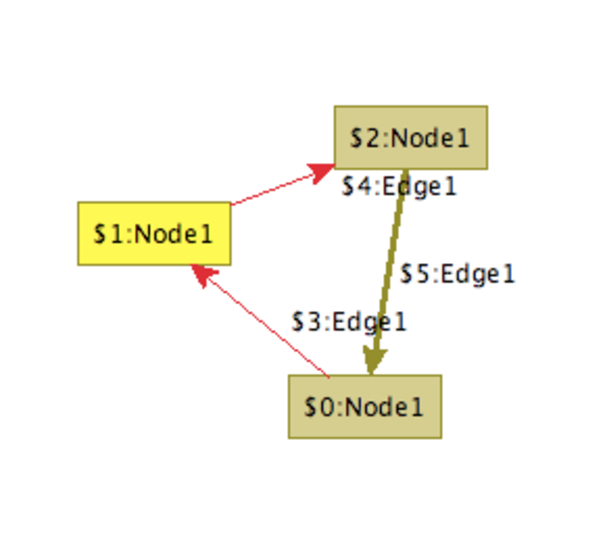
\includegraphics[width=0.25\linewidth]{fig/debug1}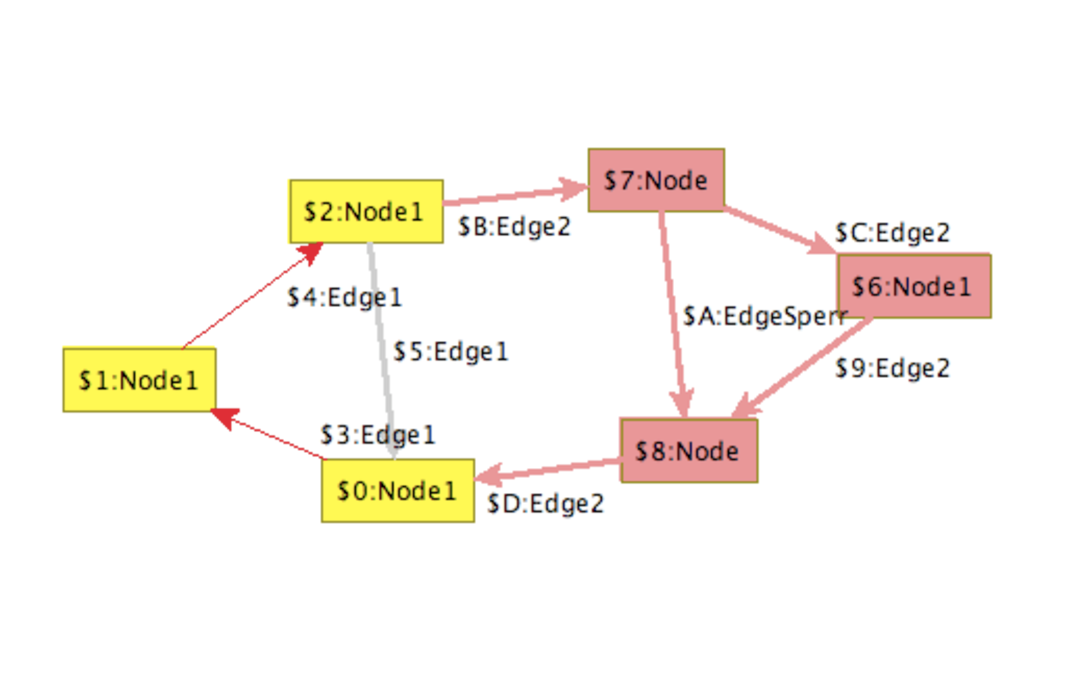
\includegraphics[width=0.4\linewidth]{fig/debug2}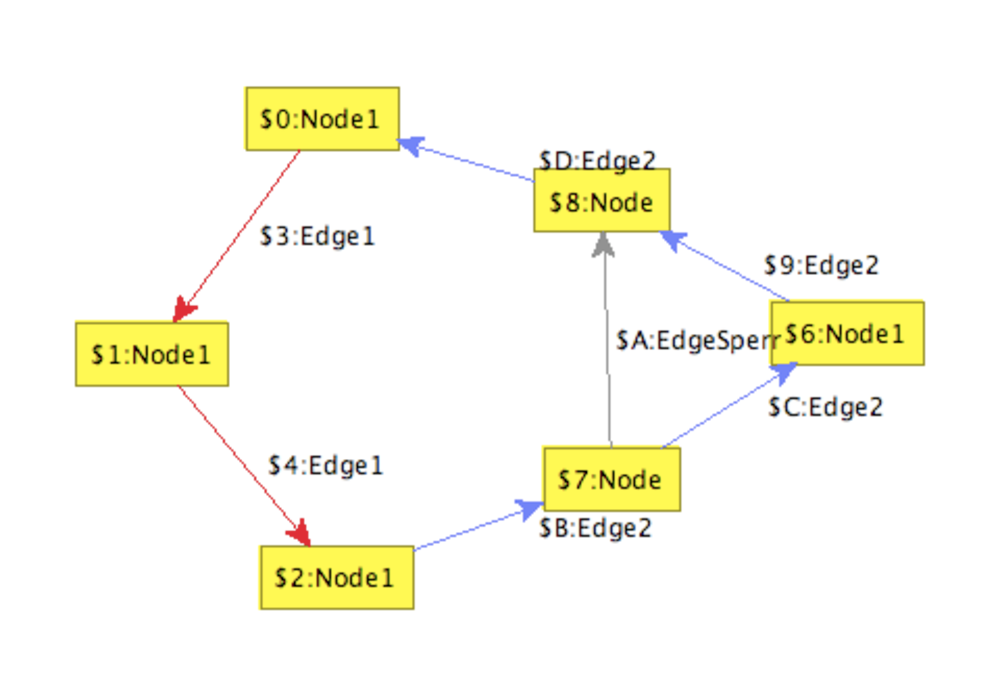
\includegraphics[width=0.4\linewidth]{fig/debug3}
  \caption{Delayed step rule application.}
  \label{figdebug}
\end{figure}
\begin{table}[htbp]
  \centering
  \begin{tabular}{|l|l|} \hline
    \textbf{Command} & \textbf{Active rule} \\ \hline
    \texttt{s} & \texttt{makeFlake1} \\
    \texttt{o} & \texttt{beautify} \\
    \texttt{s} & \texttt{doNothing} \\
    \texttt{s} & \texttt{beautify} \\ 
    \texttt{n} & \texttt{beautify} \\ 
    \texttt{o} & \texttt{makeFlake2} \\
    \texttt{r} & --- \\ \hline
  \end{tabular}
  \caption{Debug commands on \texttt{grs (makeFlake1* ; (beautify ; doNothing)* ; makeFlake2* ; beautify*)}}
  \label{tabdebug}
\end{table}
\begin{example}   
We demonstrate the debug commands with a slightly adjusted script for the Koch snowflake from \GrG's examples (see also \ref{fractals}). The graph rewriting sequence is
\begin{grshell}
debug grs (makeFlake1* ; (beautify ; doNothing)* ; makeFlake2* ; beautify*){1}
\end{grshell}
\yComp\ will be opened with an initial graph (resulting from \texttt{grs init}):
\begin{center}
  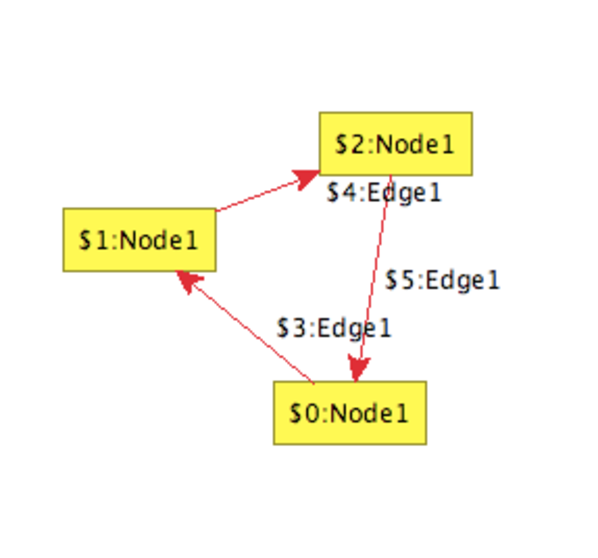
\includegraphics[width=0.3\linewidth]{fig/debug0}
\end{center}
We type \texttt{d}(elayed step) to apply \texttt{makeFlake1} step by step resulting in the graphs of figure \ref{figdebug}.
Table \ref{tabdebug} shows the effect of further debug commands.
\end{example}   


\section{LGSPBackend Custom Commands}
\label{custom}
The LGSPBackend supports the following custom commands:

\subsection{Graph Related Commands}
\begin{rail}
  'custom' 'graph' analyzegraph
\end{rail}
Analyzes the current working graph. The analysis data provides vital information for efficient search plans. Analysis data are available as long as \GrShell\ is running, i.e.\ when the working graph changes the analysis data is still available but maybe obsolete.

\subsection{Action Related Commands}
\begin{rail}
  'custom' 'actions' gensearchplan Action
\end{rail}
Creates a search plan for the rewriting rule \emph{Action} using a heuristic method and the analyze data (if the graph has been analyzed by \texttt{custom graph analyze\_graph}). Otherwise a default search plan is used. For efficiency reasons it is recommended to do analyzing and search plan creation during the rewriting procedure. Therefore the host graph should be in a stage similar to the final result. This is kind of a rough specification. In deed there might be some trial-and-error steps necessary to get a efficient search plan. A search plan is available as long as the current rule set remains loaded. 

\begin{rail}
  'custom' 'actions' setmaxmatches Number
\end{rail}
Sets the maximum amount of possible pattern matches to \emph{Number}. This command affects the expression \texttt{[\emph{Rule}]}. For \emph{Number} less or equal to zero, the constraint is reset.

